%\documentclass[12pt, draftclsnofoot, onecolumn,letterpaper]{IEEEtran}
\documentclass[12pt, letterpaper]{article}
%\documentclass[12pt, letterpaper]{IEEEtran}
\usepackage{ multirow }
\usepackage{longtable}
\usepackage{geometry}
\usepackage{ragged2e}
\usepackage[table]{xcolor}
\usepackage{booktabs}
\usepackage{graphicx}
\usepackage{caption}
\usepackage{subcaption}
\usepackage{lipsum}
\usepackage{makeidx}
\usepackage{enumerate}
\usepackage{color}
\usepackage{refstyle}
\usepackage{cite}
\usepackage{amsmath}
\usepackage{amssymb}
\usepackage{nomencl}
\usepackage{amsmath}
\usepackage{multirow}
\usepackage{graphicx}
\usepackage{multirow}
\usepackage{anysize}
\usepackage{float}
\usepackage{epstopdf}
\usepackage{threeparttable}
\usepackage{multicol}
\usepackage{amssymb}
\usepackage{adjustbox}
\usepackage{hyperref}
%\usepackage[none]{hyphenat}
%\usepackage{float}

%\usepackage{fixltx2e}
\usepackage{amsmath, amssymb, upgreek, amsthm}
\usepackage{graphicx}
\usepackage{tikz}
\geometry{letterpaper, left=20mm, right=20mm, top=20mm, bottom=20mm}
\usetikzlibrary{patterns} % LATEX and plain TEX when using Tik Z
\allowdisplaybreaks
\setlength{\textfloatsep}{2ex}
\usepackage{array}
\usepackage{enumitem}
\setlength{\parindent}{1 em}
\setlength{\parskip}{0.5 em}
\renewcommand{\baselinestretch}{1.25}
\def\dsd{d_\text{SD}}
\def\Rcoop{R_\text{Coop}}
\def\rhd{R_\text{HD}}
\def\rsd{R_\text{SD}}
\def\rsh{R_\text{SH}}
\def\Pcoops{\mathcal{P}^\text{Succ}_\text{Coop}}
\def\dsh{d_\text{SH}}
\def\dhd{d_\text{HD}}
\def\psibar{\overline{\mathcal{P}}^\text{Succ}_{i}}
\def\psbara{\overline{\mathcal{P}}^\text{Succ}_{1}}
\def\psbarb{\overline{\mathcal{P}}^\text{Succ}_{2}}
\def\psbarc{\overline{\mathcal{P}}^\text{Succ}_{3}}
\def\psbard{\overline{\mathcal{P}}^\text{Succ}_{4}}
\def\psbare{\overline{\mathcal{P}}^\text{Succ}_{5}}
\def\Ri{R_{i}}
\def\Ps{\mathcal{P}^\text{Succ}_\text{Direct}}
\def\frk{\mathrm{f}_{r_k}(r)}
\def\Rcoopj{R_\text{coop}^j}
\title{\bf \vspace*{-4ex} Statement of Responses to the Editor and the Reviewers of Paper-TNSM \\[-6ex]}
\date{}

\begin{document}
%\vspace*{-10ex}
%\sloppy
\maketitle
We would like to thank the editor and reviewers for their comments on our manuscript.
We hope that the modifications that we have made to the manuscript, and the responses that we have
provided herein will alleviate the reviewers' concerns. Below, please find our detailed responses to the editor and reviewers' comments and suggestions.
\\ [-3.ex]
% % % % % % % % % % % % % % % Editor % % % % % % % % % % % % % % % % % % % %


\clearpage
\noindent
\begin{longtable}{|p{0.975\textwidth}|}
\hline \hline
\Centering
\cellcolor{gray!60}
\textbf{Editor} \\
\hline \hline %\hline \hline \hline
\RaggedRight
\cellcolor{violet!15}
\textbf{\noindent  Comments to the Author} ``The paper has gone through three independent reviews and also checked by myself. The topic is interesting and there are merits. But there are some major concerns on the contribution, the assumption, the model derivation, and the experimental results. I hope the review comments are useful for further improving the quality of the paper. I'd therefore recommend the Resubmission''\\
\hline
\end{longtable}

\vspace*{-1\baselineskip}
\noindent \textbf{Response:\\}
We would like to thank the editor for his comment on our manuscript and giving us the opportunity to resubmit it. We have utilized the comments to improve our paper and eliminate the problems.

%\begin{longtable}{|p{0.975\textwidth}|}
%\hline \hline
%\RaggedRight
%\cellcolor{green!10}
%[1] F. Patolsky, B. P. Timko, G. Yu, Y. Fang, A. B. Greytak, G. Zheng, and C. M. Lieber, ``Detection, stimulation, and inhibition of neuronal signals with high-density nanowire transistor arrays,'' Science, vol. 313, no. 5790, pp. 1100-1104, 2006.
%\\
%\hline
%\end{longtable}




% % % % % % % % % % % % % % % Reviewer 1 % % % % % % % % % % % % % % % % % % % %
\clearpage
\noindent
\begin{longtable}{|p{.975\textwidth}|}
\hline \hline %\hline \hline \hline
\Centering
\cellcolor{gray!60}
\textbf{Reviewer 1} \\
\hline \hline %\hline \hline \hline
\RaggedRight
\cellcolor{violet!15}
\textbf{\noindent Comments to the Author} ``
The paper proposes resolving the problem of resource allocation to network slices by using a new algorithm applied to the reformulation of the problem. The results seem promising but the paper has some issues. ''\\
\hline
\end{longtable}
\vspace*{-1\baselineskip}
\noindent \textbf{Response:\\}
We would like to thank the reviewer for the careful and thorough reading of this manuscript. We hope that the responses provided herein can alleviate the reviewer's concerns.

\begin{longtable}{|p{0.975\textwidth}|}
\hline \hline
\RaggedRight
\cellcolor{gray!15}
\textbf{\noindent Comment1:} ``First, the structure of the paper makes it somewhat hard to follow and there are some mistakes in the text. A proofread is required before it can be accepted for publication.   ''\\
\hline
\end{longtable}
\vspace*{-1\baselineskip}
\noindent \textbf{Response:\\}
I have changed the paper's introduction and checked the text entirely according to this comment. 





\begin{longtable}{|p{0.975\textwidth}|}
\hline \hline
\RaggedRight
\cellcolor{gray!15}
\textbf{\noindent Comment 2:} ``Although the paper demonstrates its claims, the relaxation of conditions from the original problem formulation is not well justified. It is not clear why the initial formulation of the problem is not feasible and the reformulated makes it feasible while retaining some level of quality of the solutions given. A deeper analysis of both formulations must be presented. ''\\
\hline
\end{longtable}
\vspace*{-1\baselineskip}
\noindent \textbf{Response:\\}
The problem (13) is feasible and has feasibility points that are discussed in subsection  IV-B, and we introduce a fast algorithm (algorithm 3) for feasibility points. Although the problem is feasible, it is not convex and difficult to solve.. Since problem (13) is mixed-integer nonlinear programming with two integer constraints which are a binary variable ($e$ shows the PRB assignment) and an integer variable ($M_s$ indicate the number of VNFs in slice s), the problem is NP-hard. Solving the problem is complex. To solve the problem by inspiring Stackelberg, we reformulate the equation (13g) to reduce one of the variables ($M_s$) that can be solved after obtaining the rate of UEs ($M_s$ is similar to followers in Stackelberg Competition and power and PRB assignment is similar to leader). So, the new problem has two variables of power and PRB assignment. This new problem is convex by relaxing the binary variable (PRB assignment) and estimating the lower bounds in equation (15) because the objective function and constraints of the problem are convex and can be solved by the Lagrangian function. After obtaining the power of UEs and PRB assignment, we can obtain the achievable rate of each UE so we can find the optimal number of VNFs.

We also add this response in subsection III-A.


\begin{longtable}{|p{0.975\textwidth}|}
\hline \hline
\RaggedRight
\cellcolor{gray!15}
\textbf{\noindent Comment3:} ``Moreover, the baseline and FBDR methods used in the comparison are not well introduced. They are vaguely linked to related work but not as needed. The paper must clarify the relation of the related work and the compared alternatives. The paper must also contextualize the proposal among the related work by comparing their qualities and/or performance.  ''\\
\hline
\end{longtable}
\vspace*{-1\baselineskip}
\noindent \textbf{Response:\\}
 Two different methods are used to compare with the performance of the proposed method (IABV) and show the optimality of our approach. The first one is a baseline scheme, which uses random PRB allocation. So, the allocation of PRB to each UE is random when we have low interference, but in figures with high interference, we randomly assign just one RB to each UE. Also, the association of O-RU is carried out based on distance. It means that each UE is assigned to the nearest O-RU. The optimal power is obtained using the CVX of Matlab, which uses the successive convex approximation (SCA) method since the problem is convex. 
After achieving power and other parameters, the achievable rate will be obtained and the optimal number of VNF is
achieved from the lemma (1). The second one is similar
to the fixed BBU capacity and dynamic resource allocation
(FBDR) algorithm proposed in [18]. In this work, we have services with different QoS that
contain UEs, which is similar to tenants with different QoS
that is introduced in [18]. So, we used an algorithm similar
to FBDR adapted to our conditions for comparison. Instead
of BBU in C-RAN, we have O-DU and O-CU in O-RAN.
To use the FBDR method, we should consider the fixed
BBU capacity. We assume that O-DU and O-CU have fixed
sufficient capacity in our system model. Also, our mid-haul
link (F1 link) has adequate capacity, so there will be no
issue using the FBDR method by separating BBU to O-DU
and O-CU with this assumption. In this method, PRB and power are dynamically allocated. The number of VNFs is
obtained from the simulation. The UEs are associated with the O-RU based on the quality of their channels and the
channel distance instead of using the greedy algorithm 1 (GAA algorithm ) for O-RU assignment. The figures in [18]
show that dynamic BBU capacity and dynamic resource allocation (DBDR) perform better than FBDR for the same
priority area. We will also see that our proposed algorithm performs better than FBDR in the numerical result section.

We add this response in subsection IV-A.


\begin{longtable}{|p{0.975\textwidth}|}
\hline \hline
\RaggedRight
\cellcolor{gray!15}
\textbf{\noindent Comment4:} ``Finally, the source of the values used for the parameters in the evaluation must be clarified.  ''\\
\hline
\end{longtable}
\vspace*{-1\baselineskip}
\noindent \textbf{Response:\\}

We refer to the following list of references in our numerical result for this comment:

\begin{longtable}{|p{0.975\textwidth}|}
\hline \hline
\RaggedRight
\cellcolor{green!10}
[1] 3GPP-TS-36.104-V13.3.0, “Evolved Universal Terrestrial Radio Access (E-UTRA);
Base Station (BS) radio transmission and reception
(Release 13),” 2016-03.

[2]  3GPP-TR-36.931-V13.0.0, “Technical Specification Group Radio Access Network;
Evolved Universal Terrestrial Radio Access (E-UTRA);
Radio Frequency (RF) requirements for LTE Pico Node B
(Release 13),” 2016-01.

[3] 3GPP-TS-25.101-V4.13.0, “User equipment (UE) radio transmission
and reception (FDD)(release 4),” 2006-12.

[4]E. Mohyeldin, “Minimum technical performance requirements for
imt-2020 radio interface(s),” 2020.

[5]  ETSI-TR-138-913-V14.3.0, “5G; study on scenarios and require-
ments for next generation access technologies(3GPP TR 38.913 version
14.3.0 release 14),” 2017-10.

\\
\hline
\end{longtable}

On [1] page 11, the amount of BW is explained. In [2], the noise power is represented. In [5], the author stated the amount of delay for eMBB and URLLC on pages 24 and 25. Also, on page 26, the mMTC packet size is stated. On page 25, the URLLC packet size is stated.
In [3], on page 13, table 6.1, the maximum power is stated. In [4], on page 4, the delay of URLLC and eMBB is and also the spectral efficiency of eMBB is noted.

We add these references in IV-A (references [41]-[45]).
%%%%%%%%%%%%%%%%%%%%%%%%%%%%%%%%%%%%%%%%%%%%%%%%%%%%%%%%

\clearpage
\noindent
\begin{longtable}{|p{0.975\textwidth}|}
\hline \hline
\Centering
\cellcolor{gray!45}
\textbf{Reviewer 2} \\
\hline \hline
\RaggedRight
\cellcolor{violet!15}
\textbf{\noindent Comments to the Author:} ``The paper focus on the aspect of network slicing in 5G cellular network which entails a service aware resource allocation of the different required virtual network functions (VNFs) for different slices which have different characteristics. More specifically, the paper proposes a mixed integer mathematical problem which in the original form is non-linear and hence hard to solve. To tackle this challenge the optimization problem is decomposed into two sub-problems where the solutions are not optimal however numerical investigations show that the solutions are competitive. In general, the paper is well written and structured.''\\
\hline
\end{longtable}
\vspace*{-1\baselineskip}
\noindent \textbf{Response:\\}
We would like to thank the reviewer for careful and thorough reading of this manuscript and
for the thoughtful comments and constructive suggestions, which help us to improve the quality of
this manuscript. We hope that the responses provided herein can alleviate the reviewer concerns.



\begin{longtable}{|p{0.975\textwidth}|}
\hline \hline
\RaggedRight
\cellcolor{gray!15}
\textbf{\noindent Comment 1:} ``In terms of taking the actual delay in the proposed there are some concerns which might be important for some time critical applications especially in the ultra-reliable low latency communications (URLLC) but also for different applications that fall under the enhanced mobile broadband (eMBB) generic service framework. First of all, in the paper the authors only consider processing delay and ignore propagation and transmission delay. Since multiple paths in reality could be utilized the role of the above two components might play an important role. Nevertheless, the authors need to clearly mention why those two components are not considered, saying for example are constant is not a good enough reason to be ignored since as eluded those change based on routing decisions.''\\
\hline
\end{longtable}
\vspace*{-1\baselineskip}
\noindent \textbf{Response:\\}
Considering propagation and transmission delays is straightforward to add to the system, but we do not include them for better presentation and focus on obtaining the optimal number of VNF.
In this paper, we focus only on the processing delays to find the optimal number of VNFs, and we consider the other two delays are fixed; In the following, we describe more about these two types of delays.

The propagation delay is considered when each O-RU can connect to the number of O-DUs and can select to connect to which O-DU based on the route, capacity, and priority (Also, the connections of O-DUs to O-CUs is the same as O-RU to O-DU). Therefore, different routes are added to the system to solve the routing problem, but we do not consider it since it changes the model and does not fit in this model. So, the connection between O-RUs to O-DUs is fixed and transparent. As a result, the propagation delay is fixed and does not affect the optimization problem.
The following is a brief calculation of propagation delay.
Since the distance between the O-RU to O-DU is about 10 km and also the distance between O-DU and O-CU is about 80 km. Moreover, the distance from O-CU to the network should not exceed 200 km \cite{oranD1}. so, the propagation delay is about $T^{\text{pro}} = (10 + 80 + 200)\times 10^3 /(3\times 10^8) < 1ms $. Since fronhaul, midhaul, and backhaul are fiber optics, c is the speed of light. Also, due to the edge technique in O-DU or O-CU for users with low latency, this amount of latency is greatly reduced. But we also do not focus on edge processing in this paper. You can find more about these distances in this \href{https://blogs.keysight.com/blogs/inds.entry.html/2020/06/30/5g_testing_what_is-0nzj.html\%23:~:text=The\%20data\%20requirements\%20are\%20about,DUs\%20is\%20about\%2080\%20km.}{link}.
The following is a brief calculation of transmission delay to show that it does not affect the optimization since it has such a small amount.
In URLLC and mMTC, the mean packet size can be between 20 to 32 byte; Also, the minimum data rate is assume to be $46 bits/sec/Hz \times BW (180 KHz)$. So the transmission delay from O-RU to O-DU is about $T^{fr,t} = \frac{20\times 8}{46 \times 180 \times 10^3} < 2 us$. As a result, the $T^{fr,t} \approx T^{mid,t} \approx T^{b,t}$. for eMBB, the packet size can be 100 times larger and the delay is not exceed the 0.6ms.  

We add this response in subsection II-D.



\begin{longtable}{|p{0.975\textwidth}|}
\hline \hline
\RaggedRight
\cellcolor{gray!15}
\textbf{\noindent Comment 2:} ``Also, note that for calculating processing delay requests for different services arriving at blade servers for vnf applications might get different treatment on how they access VMs or containers hence a single queue with non-priority and/or preemption (m/m/1) might not be a good approximation on the performance.''\\
\hline
\end{longtable}
\vspace*{-1\baselineskip}
\noindent \textbf{Response:\\}
The processing delay can be considered an M/M/1; since the number of arrival packets in the system is enormous, and the packets are independent. Moreover, the impact of a single packet on the system's performance is minimal. Also, the queue discipline will be first-in, first-out (FIFO), and the arrival packet is assumed to follow a Poisson process. The system's clock is constant, and the size of the tasks is not fixed. So, we suppose that service times are exponentially distributed [36]. In addition, we assume that the arrival packets of each service have the same priority, and we consider priority between services, not between UEs of one service. Because we assumed that the UEs of a service have the same priority, their sent packets also have an equal priority. Also, the services are isolated, and this priority does not invalidate the queue assumption. Furthermore, one service's priority over another can be higher, affecting the whole optimization and not queue formulation since the UEs in each service have the same priority, and each service has its processing delay independent of other services.

We add this response in subsection II-D-1.


\begin{longtable}{|p{0.975\textwidth}|}
\hline \hline
\RaggedRight
\cellcolor{gray!15}
\textbf{\noindent Comment 3:} ``Also worth noting, that later on in the problem formulation there is the notion of service priority $\delta_s$ for data rate but this seems not to be used for accessing cloud resources. For example one could have changed the optimization problem and considered average allocated transmission rate and optimize with the same priorities access to cloud resources (instead of allocating equal access to vnf resources).''\\
\hline
\end{longtable}
\vspace*{-1\baselineskip}
\noindent \textbf{Response:\\}
In this problem, since the priority is in the objective function of the equation (13), the priority has whole effect optimization.
So, priority is given to the whole optimization problem, and the optimization problem obtains the number of VNFs by affecting the priority term. If we were to discuss the placement of VNFs on the data centers, the problem would become a knapsack or bin-packing problem, and here the prioritization would affect the resource allocation algorithm, including memory, RAM, CPU, and bandwidth. So the algorithm was implemented based on prioritization.


\begin{longtable}{|p{0.975\textwidth}|}
\hline \hline
\RaggedRight
\cellcolor{gray!15}
\textbf{\noindent Comment 4:} ``Some form of rationalization should be given for abstracting Interference as Gaussian noise. This is important because we expect the system to be interference limited and cell edge users to experience significant different levels of performance compared to centre cell users.''\\
\hline
\end{longtable}
\vspace*{-1\baselineskip}
\noindent \textbf{Response:\\}
 $I_{r,u(s,i)}^{k}$ is the sum of the power of interfering signals and quantization noise represented as follow
%{\color{red} use paranthesis in the following equation to clear +}
\begin{subequations}\label{eqI}
\begin{alignat}{4}
&I_{r,u(s,i)}^{k} =\\
 &\underbrace{\sum_{\substack{l=1 \\ l\neq i}}^{{U}_{s}} e^{k}_{u(s,i)}e^{k}_{u(s,l)}  p_{u(s,l)}^{k}\sum_{\substack{r'=1 \\ r'\neq r}}^{R}|{\bold{h}_{r',u(s,i)}^{H \: k}} \bold{w}_{r',u(s,l)}^{k} g_{u(s,l)}^{r'}|^2}_{\text{(intra-slice interference)}}+\\
&\underbrace{\sum_{\substack{n = 1 \\ n\neq s}}^{S}\sum_{l=1}^{{U}_s} e^{k}_{u(s,i)}e^{k}_{u(n,l)}  p_{u(n,l)}^{k}\sum_{\substack{r'=1 \\ r'\neq r}}^{R}|{\bold{h}_{r',u(s,i)}^{H \: k}} \bold{w}_{r',u(n,l)}^{k} g_{u(n,l)}^{r'}|^2}_{\text{(inter-slice interference)}}\\
&+\underbrace{  \sum_{j=1}^{{R}} {\sigma_q}^2 |\boldsymbol{h}_{r,{u(s,i)}}^k|^2 }_{\text{(quantization noise)}},
\end{alignat}
\end{subequations}
%{\color{red} $\gamma_1$ is constant used instead of variable. }
%where $\gamma_{1} = e^{k}_{u(s,i)}e^{k}_{u(s,l)}$ and $\gamma_{2} = e^{k}_{u(s,i)}e^{k}_{u(n,l)}$.
where $e^{k}_{u(s,i)}$ is the binary variable to show whether the $k^{th}$ PRB is allocated to the UE $i$ in slice $s$, assigned to $r^{th}$ O-RU. %($\gamma_1$ and $\gamma_2$ are two variales. You  define on variable here.)
Furthermore, there is no inter-slice interference since slices are isolated and there is just intra-slice interference.

Here we have two Gaussian noise types: additive Gaussian noise and the other is Gaussian quantization noise. The second noise is added to the interfering signal and shown with $ I_{r,u(s,i)}^{k}$ and it is different with interference.
To obtain SNR as formulated in \eqref{eq1}, let $y_{u(s,i)} $ be the received signal of UE $i$ in $s^{th}$ service formulated as
\begin{equation}\label{eq2}
y_{u(s,i)} = \sum_{r = 1}^{R}\sum_{k=1}^{K_s} \boldsymbol{h}^{H \: k}_{r,u(s,i)} g_{u(s,i)}^r e^k_{r,u(s,i)}{x_Q}^k_{r,u(s,i)}+ z_{u(s,i)},
\end{equation}

%\boldsymbol{w}^k_{r,u(s,i)}p^k_{r,u(s,i)}  $\mathfrak{y}^k_{r,u(s,i)} =\boldsymbol{w}^k_{r,u(s,i)}{p^{k \: \frac{1}{2}}_{r,u(s,i)}} x_{u(s,i)}+ \boldsymbol{q}_{r}$
where ${x_Q}^k_{r,u(s,i)} ={x_P}^k_{r,u(s,i)}+ \boldsymbol{q}_{r}$. Also, ${x_P}^k_{r,u(s,i)}= \boldsymbol{w}^k_{r,u(s,i)}{p^{k \: \frac{1}{2}}_{r,u(s,i)}} x_{u(s,i)} $, and  $ x_{u(s,i)}$ depicts the transmitted symbol vector of UE $i$ in $s^{th}$ set of service,  $z_{u(s,i)}$ is the additive Gaussian noise $z_{u(s,i)} \backsim \mathcal{N}(0,N_0)$ and $N_0$ is the noise power.
Moreover, ${x_P}$ denotes the precoded message before compression, and ${x_Q}$ illustrates the precoded message after compression that is shown in figure \ref{fig:pq}. 
In addition, $\boldsymbol{q}_{r} \in \mathbb{C}^{J }  $ indicates the quantization Gaussian noise 
($\boldsymbol{q}_{r} \backsim \mathcal{N}(0,{\sigma_q}^2\boldsymbol{I_{R}} )$), which is made from signal compression in O-DU.
\begin{figure}
  \centering 
  \captionsetup{justification=centering}
    \includegraphics[scale = 0.7]{Qdiag.png}
    %\includegraphics[max height=30cm,max width=9.5cm]{Drawing15.eps}
    %\includegraphics[width=\textwidth]{finalDraw.pdf}
  \caption{Precoding and Quantization of Signal}
  \label{fig:pq}
\end{figure}

We add this response in subsection II-B.


\begin{longtable}{|p{0.975\textwidth}|}
\hline \hline
\RaggedRight
\cellcolor{gray!15}
\textbf{\noindent Comment 5:} ``Constraint 13n (changed to 13k in new version) is not clear - it means that there are VMs and/or containers available in the network and an operator denies service due to an energy consumption budget (which again is not very detailed to capture the actual energy consumption of each node/vnfs under different loads etc.). In general the subsection on VNF power consumption is very limited in scope. ''\\
\hline
\end{longtable}
\vspace*{-1\baselineskip}
\noindent \textbf{Response:\\}
{A significant issue facing the industry is reducing energy consumption. Data centers are one of the most energy-consuming. As a result, restrictions are placed on data centers' energy, including virtual machines (VMs). So, one of our goals is to limit the energy consumption of total VNFs that can be run as VM on data centers. So, by applying a custom policy on total power consumption, we can control data centers' power consumption ($\phi^{\text{\text{tot}}}  \leq \phi^{max}$).

We add this response in subsection II-E.

\clearpage
\noindent
\begin{longtable}{|p{0.975\textwidth}|}
\hline \hline
\RaggedRight
\cellcolor{gray!15}
\textbf{\noindent Comment 6:} ``Some rationalization is needed on why the packet size is considered to be 20 bytes. ''\\
\hline
\end{longtable}
\vspace*{-1\baselineskip}
\noindent \textbf{Response:\\}

We refer to the following reference in our numerical result for this comment:

\begin{longtable}{|p{0.975\textwidth}|}
\hline \hline
\RaggedRight
\cellcolor{green!10}
[1]  ETSI-TR-138-913-V14.3.0, “5G; study on scenarios and require-
ments for next generation access technologies(3GPP TR 38.913 version
14.3.0 release 14),” 2017-10.

\\
\hline
\end{longtable}

On [1], on page 25, the URLLC packet size is stated to be 32 bytes, and on page 26, the packet size of mMTC is stated to be 20 bytes. We have changed the URLLC packet size to 32, but it has very little impact on the simulation result. 

We add this reference in IV-A (reference [45]).

\begin{longtable}{|p{0.975\textwidth}|}
\hline \hline
\RaggedRight
\cellcolor{gray!15}
\textbf{\noindent Comment 7:} ``Comparison with [18] might not be fair since that work also considers BBU capacity and also performs admission control functionalities, also there are different tenants that have different users with variable required QoS. ''\\
\hline
\end{longtable}
\vspace*{-1\baselineskip}
\noindent \textbf{Response:\\}
We use a method which is similar to the fixed BBU capacity and dynamic resource allocation (FBDR) algorithm proposed in [18]. In this work, we have services with different QoS that contain UEs, which is similar to tenants with different QoS that is introduced in [18].
 So, we used an algorithm similar to FBDR adapted to our conditions for comparison.  
Instead of BBU in C-RAN, we have O-DU and O-CU in O-RAN. To use the FBDR method, we should consider the fixed BBU capacity. We assume that O-DU and O-CU have fixed sufficient capacity in our system model. Also, our mid-haul link (F1 link) has adequate capacity, so there will be no issue using the FBDR method by separating ‌BBU to O-DU and O-CU with this assumption.
In this method, PRB and power are dynamically allocated. The number of VNFs is obtained from the simulation. The UEs are associated with the O-RU based on the quality of their channels and the channel distance instead of using the greedy algorithm 1 (GAA algorithm ) for O-RU assignment.

We add this response in subsection IV-A.


\begin{longtable}{|p{0.975\textwidth}|}
\hline \hline
\RaggedRight
\cellcolor{gray!15}
\textbf{\noindent Comment 8:} ``Also, interference is measured in a more detailed manner (maximum interference per UE) and hence when this relaxed (Guassian noise) the performance expected to slightly increase. Hence, some more detailed discussion on what has been assumed is needed. ''\\
\hline
\end{longtable}
\vspace*{-1\baselineskip}
\noindent \textbf{Response:\\}
Here we have two Gaussian noise types: additive Gaussian noise and the other is Gaussian quantization noise which is shown in Fig \ref{fig:pq}. We offer the sum of interference and the Gaussian quantization noise with $ I_{r,u(s,i)}^{k}$. Also, the Gaussian quantization noise is independent of interference and related to channel gain of UEs.

We add this response in subsection II-B.
%%%%%%%%%%%%%%%%%%%%%%%%%%%%%%%%%%%%%%%%%%%%%%%%%%%%%%%%%

\clearpage
\noindent
\begin{longtable}{|p{0.975\textwidth}|}
\hline \hline
\Centering
\cellcolor{gray!45}
\textbf{Reviewer 4} \\
\hline \hline
\RaggedRight
\cellcolor{gray!15}
\textbf{\noindent Comment 1:} ``The description of  ``unhealthy neuron'' or ``neurons that have lost their ability to communicate'' and the nano-machines to connect them seems to provide a possible future application to the communication channel model proposed. What the manuscript is not fully analyzing in the opinion of this reviewer is exactly how the nano-machines could utilize this model from an engineering perspective. If this connection is not considered to be the focus and therefore was not researched, then the consideration should be made to remove the concept of nano-machines from the ``System Model'' section (and subsequent sections) and use it merely for motivating the model.''\\
\hline
\end{longtable}
\vspace*{-1\baselineskip}
\noindent \textbf{Response:\\}
We would like to thank the reviewer for careful and thorough reading of our manuscript and for
the thoughtful comments and constructive suggestions, which helped us to improve
the quality of this manuscript. We hope that the modifications that we have made to the manuscript, and the
responses that we have provided herein will alleviate the reviewer concerns.

In recent years, engineering applications of nano-technology have also been investigated with increasing interest
for the design of bio-inspired intelligent nano-devices or nano-machines connected in a network. In this manuscript, we considered the concept of nano-machines in the proposed system model according to the reported efforts to interface the neuron's body
with synthetic nano-scale materials in the literature. We provide a brief explanation in the following. We refer to the following list of references in our explanation in this comment:


\clearpage
\begin{longtable}{|p{0.975\textwidth}|}
\hline \hline
\RaggedRight
\cellcolor{green!10}
[1] F. Patolsky, B. P. Timko, G. Yu, Y. Fang, A. B. Greytak, G. Zheng, and C. M. Lieber, ``Detection, stimulation, and inhibition of neuronal signals with high-density nanowire transistor arrays,'' Science, vol. 313, no. 5790, pp. 1100-1104, 2006.

[2] N. Sakai, J. Mareda, and S. Matile, ``Ion channels and pores, made from scratch,'' Molecular BioSyst., vol. 3, pp. 658-666, 2007.

[3] P. Gorostiza and E. Isacoff, ``Optical switches and triggers for the manipulation of ion channels and pores,'' Molecular BioSyst., vol. 3, pp. 686-704, 2007.

[4] Mesiti, Fabio, and Ilangko Balasingham. ``Nanomachine-to-neuron communication interfaces for neuronal stimulation at nanoscale.'', IEEE Journal on Selected Areas in Communications, vol. 31, no. 12, pp. 695-704, 2013.

[5] N. Rouach, E. Avignone, W. Même, A. Koulakoff, L. Venance, F. Blomstrand, and C. Giaume, ``Gap junctions and connexin expression in the normal and pathological central nervous system,'' Biology Cell, vol. 94, no. 7-8, pp. 457-475, 2002.

[6] J. Hjorth, K. T. Blackwell, and J. Hellgren Kotaleski, ``Gap junctions between striatal fast-spiking interneurons regulate spiking activity and synchronization as a function of cortical activity'', J. Neuroscience, vol. 29, no. 16, pp. 5276-5286, 2009.

[7] R. D. Traub, M. A. Whittington, E. H. Buhl, F. E. N. LeBeau, A. Bibbig, S. Boyd, H. Cross, and T. Baldeweg, ``A possible role for gap junctions in generation of very fast EEG oscillations preceding the onset of, and perhaps initiating, seizures,'' Epilepsia, vol. 42, no. 2, pp. 153-170, 2001.
\\
\hline
\end{longtable}


\clearpage
In [1], the authors described the successful attempt to interface nano-wire (NW) FET transistors (SiNW-neurons) with soma, dendrites and axon, allowing high precision measurement and
stimulation with an array of 50 NW connections per neuron. The synthesis of ion channels and pores, assembled artificially by chemical composition were reported in [2], whereas synthetic nano-scale actuators (nano-toggles, nano-keys and nano-tweezers) to manipulate ion channels were proposed in [3].
Hence, the advances in the molecular manipulation of the matter can allow the fabrication of bio-inspired SnM interfaces.
Upon these considerations and the available nano-technology, the authors in [4] identified a set of possible SnM interface implementations. We employed one type of these interfaces in our system model according to [4] which is denoted as Gap Junction Interface.


\textbf{Gap Junction Interface [4]}:

With gap junctions, two cellular membranes in direct contact are separated by only 3 nm and for each side, clusters of \textit{connexine} (Cx36) proteins [5], combine to form a channel with diameter 1-2 nm, the \textit{connexine}, allowing bidirectional flows of ions (currents) between cells. Synthetic connexines assembled \textit{in-situ} by SnMs could allow the opening of additional ion channels on the membrane, enhancing the neuronal activity. In the following figure [4], a sample scenario with multiple SnMs attached to the target neuron is depicted. This method is motivated and supported by neuro-scientific studies [6], [7] reporting the important role of gap junctions in \textit{oscillatory behaviors} and \textit{synchronization} phenomena between neurons.

\begin{figure}[H]
\centering
\includegraphics[width=.78\textwidth,height=.3\textheight]{Gap.png}
\caption{ Diagram of a SnM based on gap junctions. The neuronal membrane is in contact with each SnM, establishing additional connexone channels which allow the flow of ions and currents [4].}
\label{new_1}
\end{figure}










\end{document}


